% ========================================================
% INTRO
% ========================================================
\section{Introduction}\label{s20}
The Compact Pixel Tracking Telescope has two different versions that were both constructed at \ac{ETH} in Z{\"u}rich. It is called telescope due to the fact that it utilises different single planes to get information about a \ac{DUT}. Its main purpose is to provide an event trigger and high resolution tracks.\\ 
To accomplish that goal it consists of several single \ac{CMS}-Pixel chips that are placed consecutively, perpendiclar to the beam. The chips are mounted on so-called adapter planes and have a fixed distance to one another that is given by the connectors of the connectors of the motherboard.\\
The planes are daisy chained and are read out by the \ac{DTB} which makes them accessible via a computer.
% ========================================================
% 1
% ========================================================
\section{Telescope Layout}\label{s21}
As already mentioned above, there are two versions of the telescope. Version 1 was designed to be as simple as possible and consists of six planes with analogue chips. Whereas the second version that was built on the experience with first one, comprises three plane modules, which may be combined to bigger modules. The modules of version 2 can consist either of digital chips or of analogue chips. Version 2 has some additional features as well that will be mentioned in the following.\\
Both consist mainly of three parts: a motherboard, adapter planes and the \ac{ROC}s.
% ========================================================
\subsection{Motherboard}\label{s210}
The motherboard is the main frame of the telescope. Pictures of the motherboards are shown in \ar{pmb}, the number in square bracket in the following text refer to the numbers in the pictures.\par
\begin{figure}[h]
	\centering
	\subbottom[Version 1]{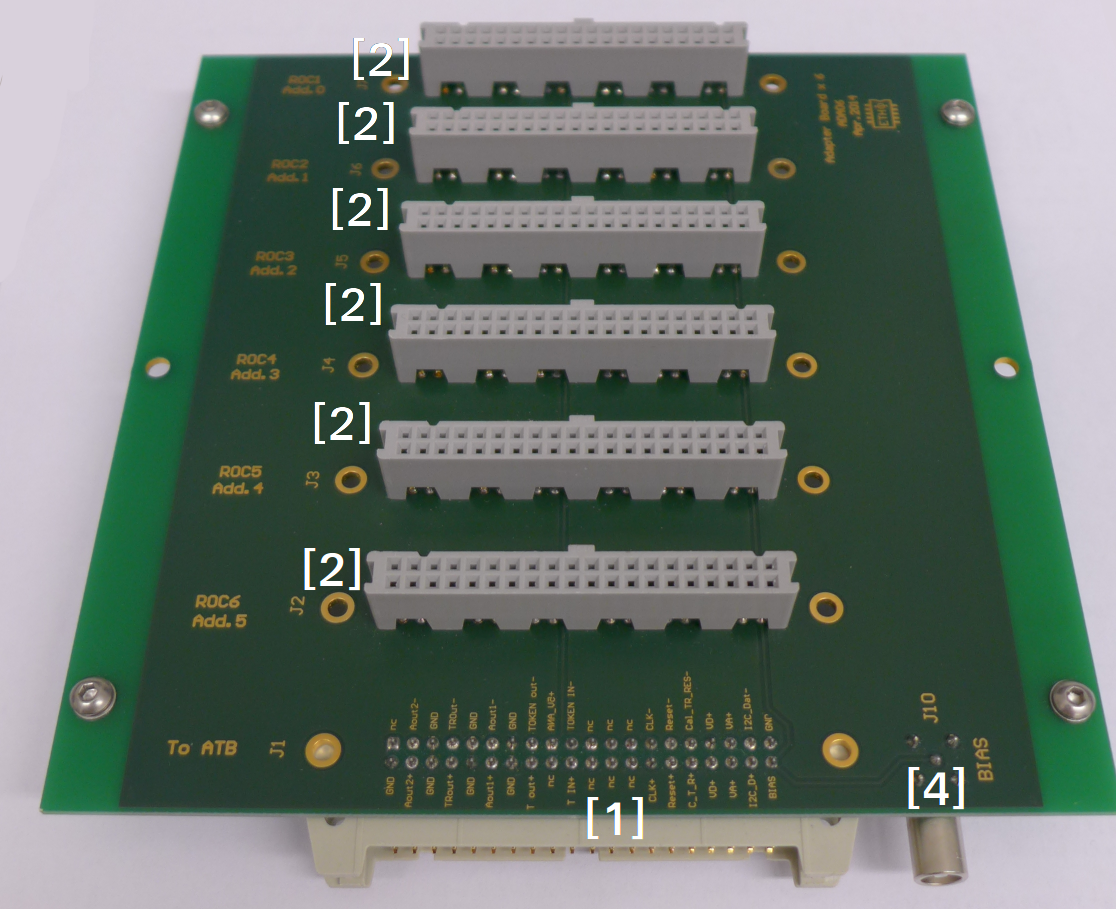
\includegraphics[width=0.52\textwidth]{setup/mb1}\label{p0}}
	\hfill
	\subbottom[Version 2]{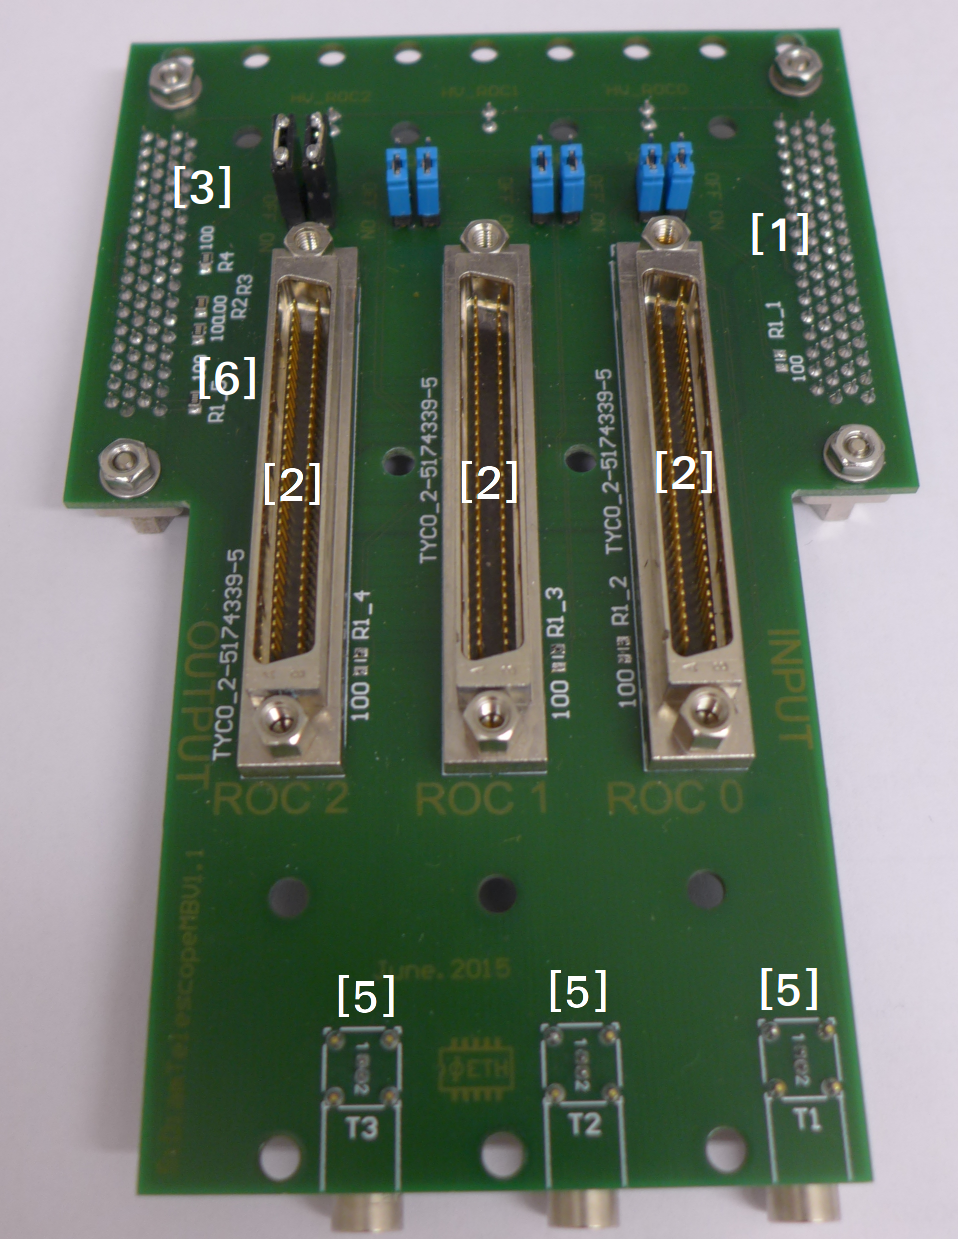
\includegraphics[width=0.42\textwidth]{setup/mb2}\label{p1}}
	\caption{The motherboards of the two telescopes}
	\label{pmb}
\end{figure}\no
The \ac{PCB} has a male connector [1] for a data transfer cable to communicate with a test board. In case of version 2 there is a second male [3] connector to which another telescope may be connected and that can only be used only as an output of the data stream. Next in line after the input come several daisy chained female connectors [2] to plug in the adapter planes. In order that the token can be sent through the whole chain, either the planes have to be plugged into [2] or a token jumper (\ar{pjumper}) has to be used. In addition version 1 has a LEMO connector [4] that allows to bias all of the connected sensors and version 2 has a differential LEMO outputs [5] for the fast-OR of every plane. All signals that pass through the telescope are properly terminated by resistors on the motherboard\footnote{In case of version 1 the resistors are underneath the board}. In case of version 2 there are boards with and without resistors and one should take care that only the last board in the chain is one with termination. Otherwise the signals might get too low to be measured.\\
The main differences of the two versions are stated in \ar{t1}.\\
The version 1 of the telescope was limited to a maximum of six static analogue planes. A main advantage of the other version is its flexibility to chain multiple three-plane telescopes together. Furthermore it easier and more convenient to place the token jumpers now. The Dimensions of the two telescopes are shown in \ar{pdim}.
\begin{table}[ht]
	\begin{tabularx}{\textwidth}{X|c|c}
		\noalign{\hrule height 2pt}
										& Version 1 			& Version 2 					\\\hline
		Connector type 					& ATA 40 pin 			& VHDCI 68 pin					\\			
		Number of planes per telescope 	& $6$ 					& $3$							\\
		Maximum number of Planes per read out chain		& $6$					& $3\times3$ \footnotemark[2] \\
		Fast-OR	output					& directly on the plane	& on the motherboard			\\
		Token jumper					& \ar{pjumper1}				& \ar{pjumper2}	\\
		\noalign{\hrule height 2pt}
	\end{tabularx}					
	\caption{Differences between the two motherboard versions}
	\label{t1}
\end{table}\no
\footnotetext[2]{Theoretically one could chain an infinite amount of telescopes. In reality the timing between the planes gets worse the longer the data has to travel, s.t. it not possible to read out more than three connected telescopes.}
\begin{figure}[ht]
	\centering
	\subbottom[Version 1: Self crafted token jumper by hard wiring the token line of a spare ATA connector. This jumper is then placed on the connector of the motherboard instead of a plane.]{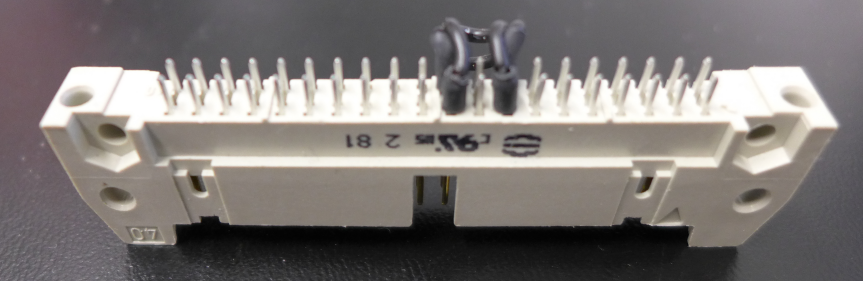
\includegraphics[width=0.47\textwidth]{TokenJumper}\label{pjumper1}}
	\hfill
	\subbottom[Version 2: The blue jumpers loop the token into the plane and the black jumpers make the token pass the plane. A blue jumper at the ``Out'' position will send the token into the next connected motherboard and a black one back to the \ac{DTB}]{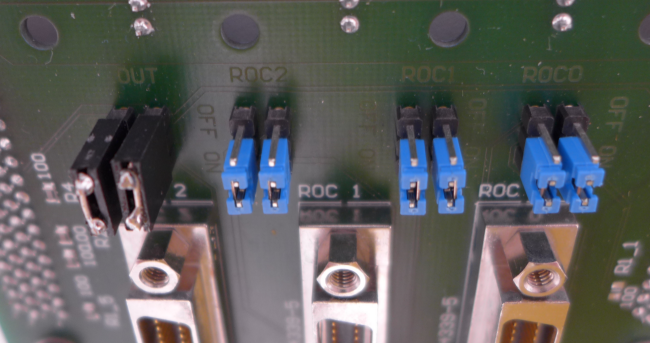
\includegraphics[width=0.47\textwidth]{setup/jumper2}\label{pjumper2}}
	\caption{The token jumpers for the two version of the telescope.}
	\label{pjumper}
\end{figure}\no
\begin{figure}[ht]
	\centering
	\subbottom[Version 1]{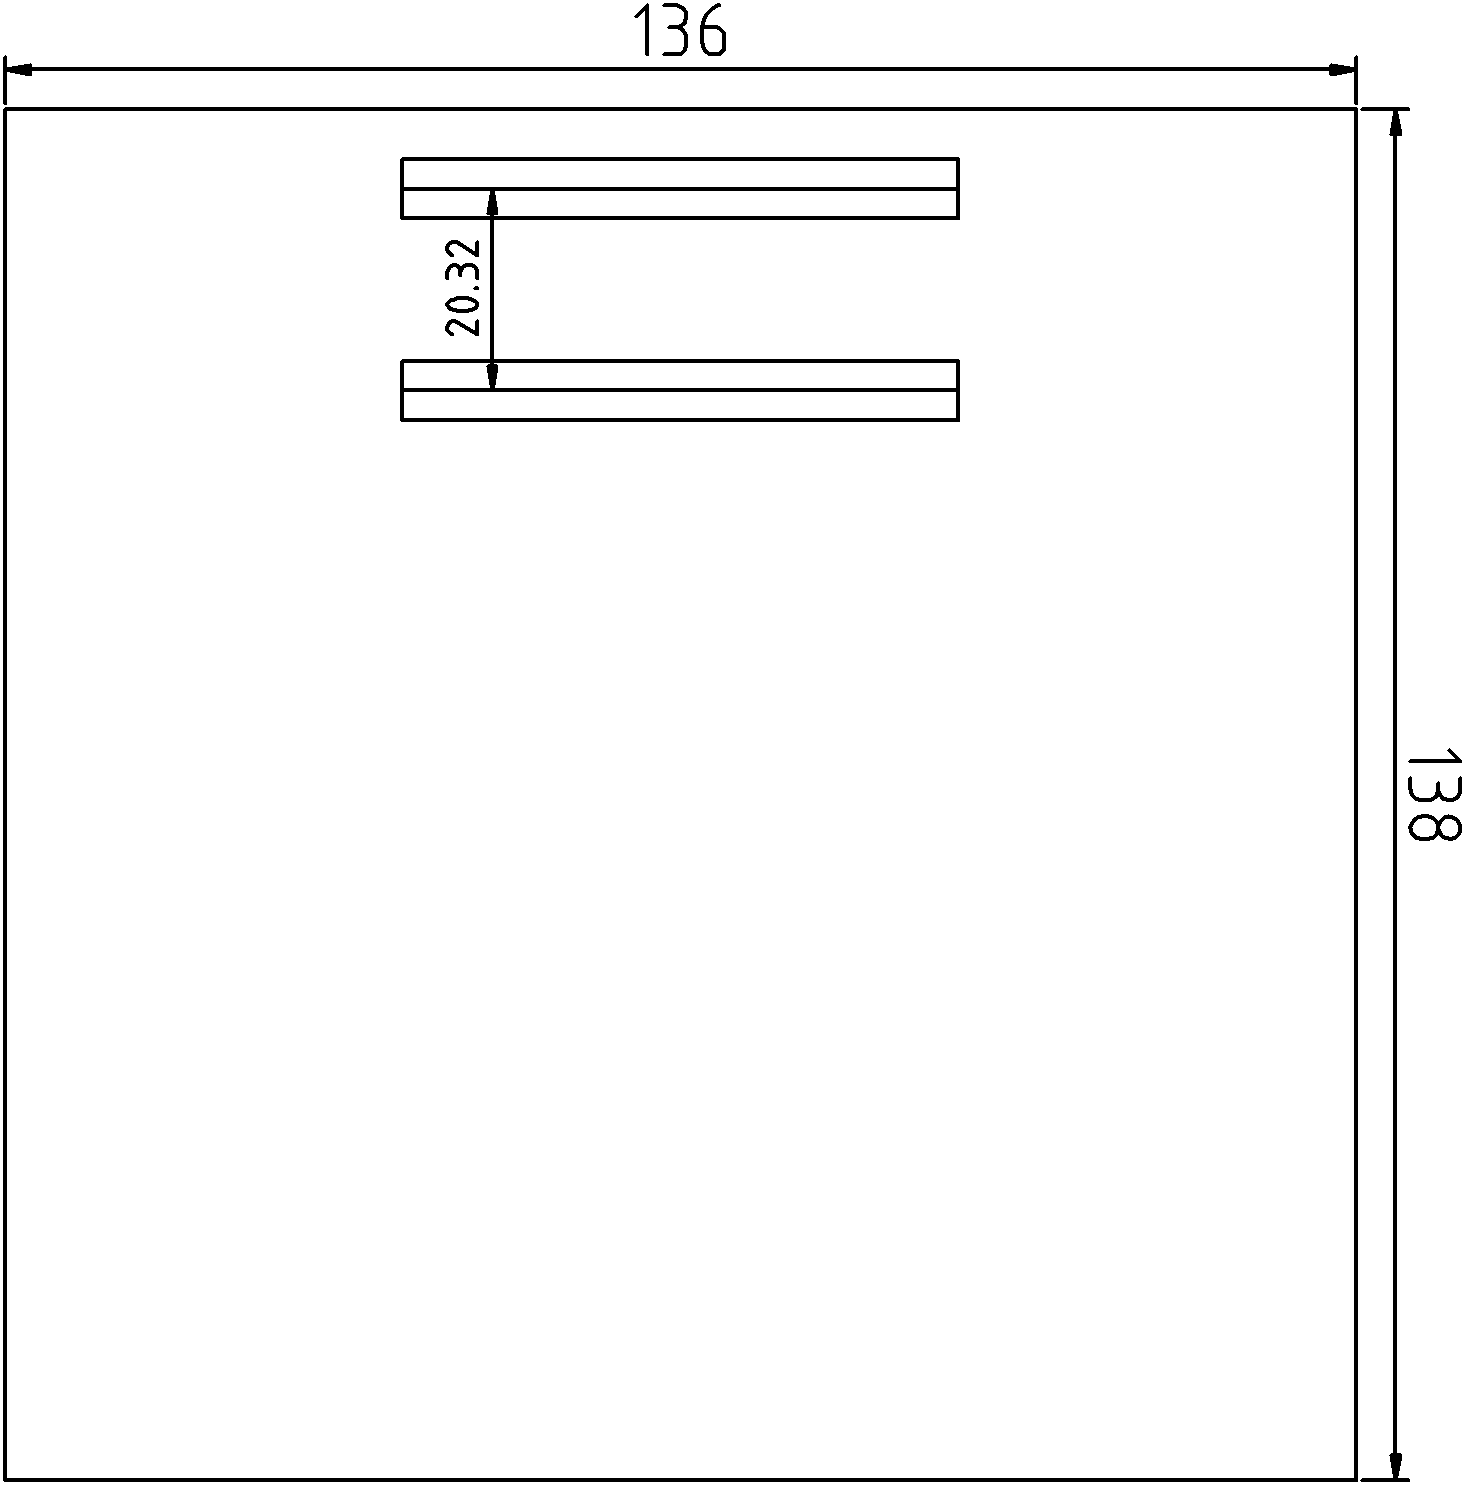
\includegraphics[width=0.47\textwidth]{dim1}\label{pdim1}}
	\hfill
	\subbottom[Version 2]{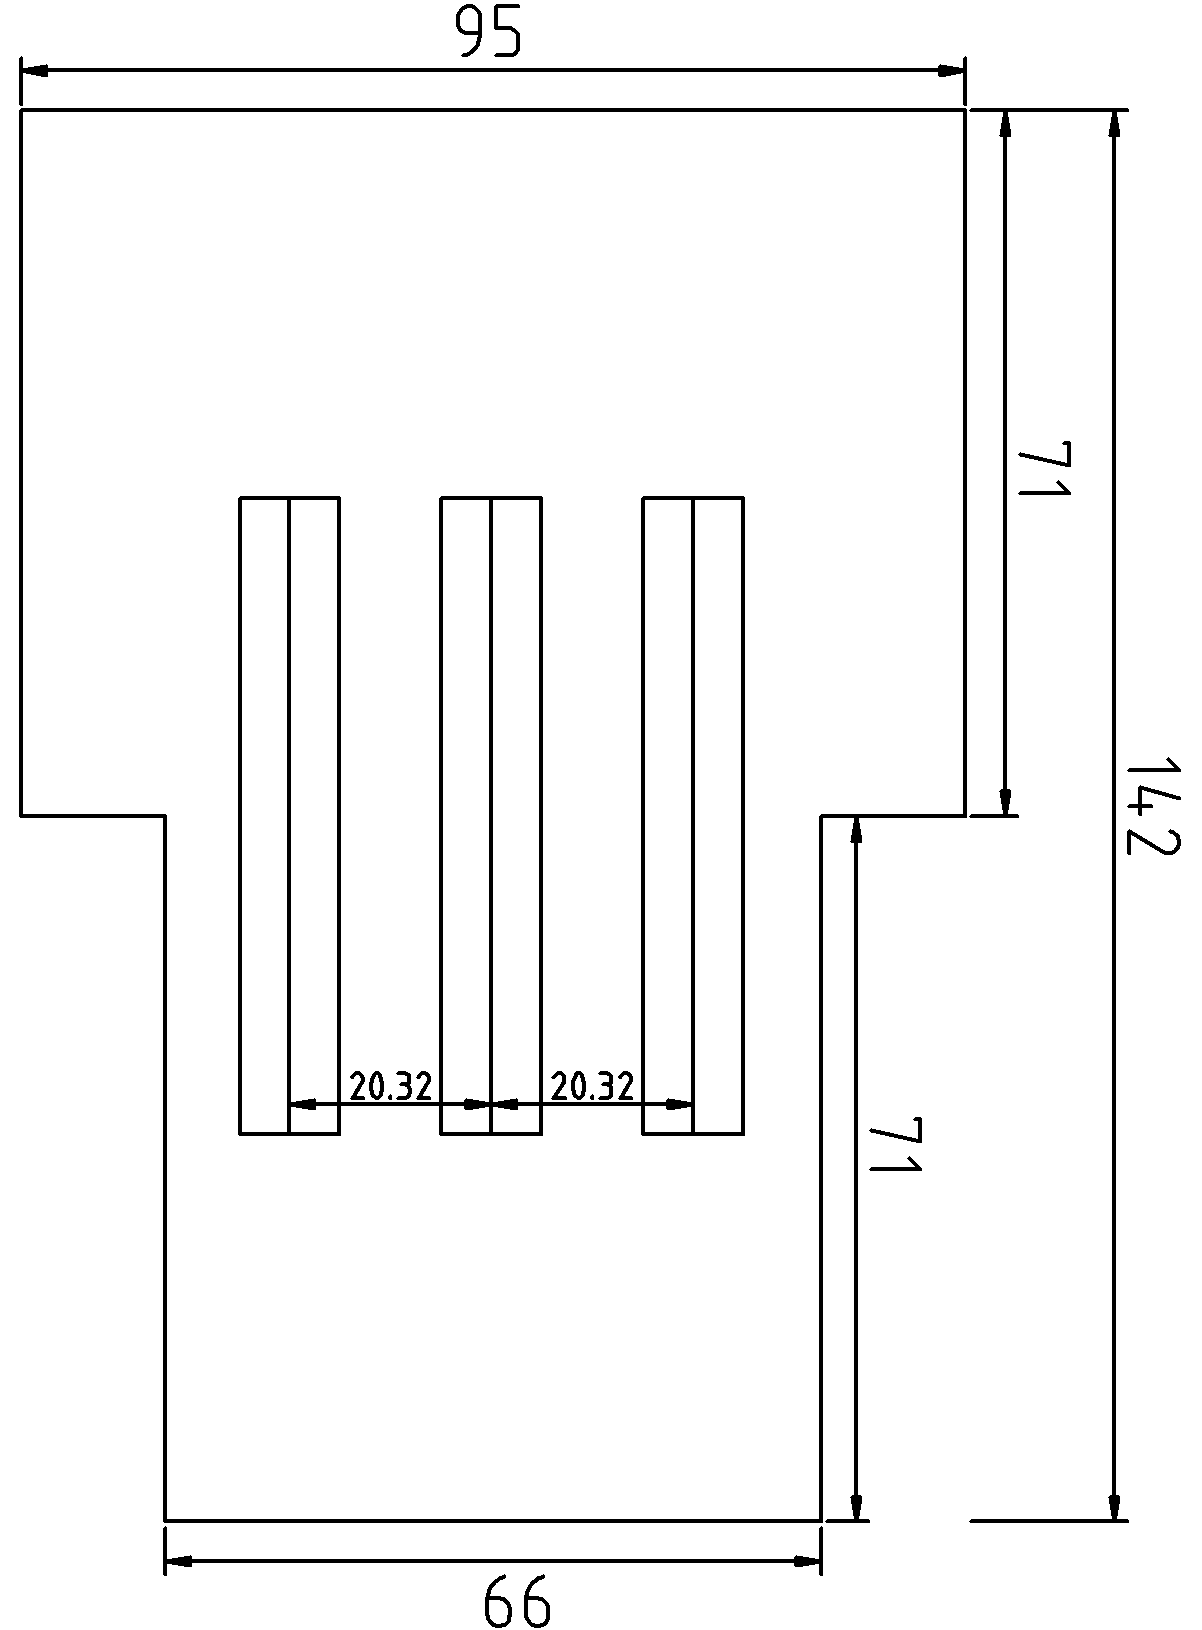
\includegraphics[width=0.47\textwidth]{dim2}\label{pdim2}}
	\caption{Dimensions of the two motherboards in millimetres.}
	\label{pdim}
\end{figure}\no
% ========================================================
\newpage
\subsection{Adapter Plane}\label{s211}
The adapter plane is the link between the telescope and a single \ac{CMS}-Pixel 
\begin{wrapfigure}{r}{5cm}
	\vspace*{-10pt}
	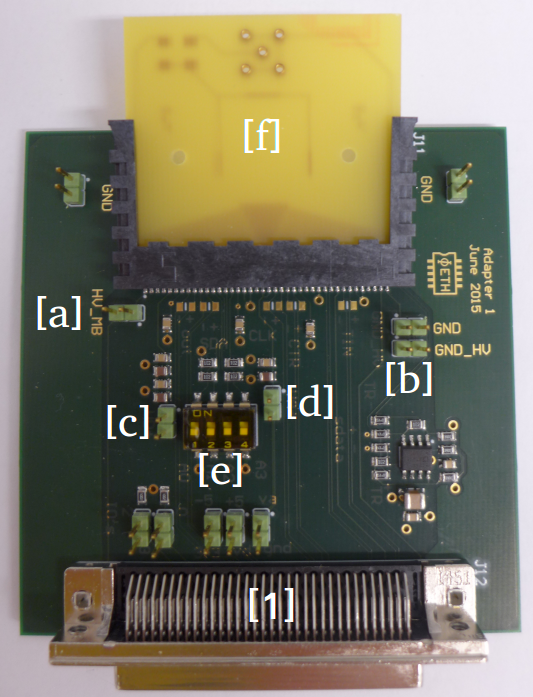
\includegraphics[width=5cm]{setup/digada}
	\caption{Digital adapter plane.}
	\label{p6}
	\vspace*{-5pt}
\end{wrapfigure} 
chip. The numbers in the following description refer to parts in \ar{p6} and \ar{padaana}. On the bottom end of the \ac{PCB} is a male connector [1] with which the plane can be plugged directly into the motherboard. The analogue planes of both telescope versions are very similar. Their differences are the already mentioned type of connector (\ar{t1}) and that there are two differential outputs for the fast-OR on the PCB of version 1 [2] (\ar{p4}) that were moved to the motherboard in version 2. Apart from that they both have an input for biasing the sensor [3], an amplifying circuit for the fast-OR [4], a small cable connector [5] to the \ac{ROC}\footnote[3]{This connector was already used for the \ac{PLT} and was kept since then.} and cable pins [6] to bias the \ac{ROC}. In version 2 there is an additional jumper [7] to allow biasing from either the adapter plane or via the connector to the motherboard. In both cases, the BIAS-GND pin of [8] has to be connected to the other outer pin of [8]. In order to bias the \ac{ROC} a cable [9] has to be connected from the BIAS- pin of [6] to the \ac{ROC} itself.\\
The adapter for the digital chips, which is shown in \ar{p6}, can only be used in combination with version 2 and differs a bit from the analogue one. The only way to bias the digital chips is via the test board and the SCSI connector, which means that there has to be a jumper at HV-MB [a] and GND-HV [b]. Likewise two jumpers have to connect the supply voltages VD [c] and VA [d] to the chip. Another very useful improvement is the dip switch box [e] in the middle of the plane, which allows to set any \ac{I2C} address between $0$ and $15$. Since the digital chips are put on special \ac{PCB}s [f], the adapter has a completely different mounting system, s.t. the chips can be easily plugged in and out, whereas the analogue \ac{ROC}s have to be screwed to the \ac{PCB}.
\begin{figure}[ht]
	\centering
	\subbottom[Version 1 without \ac{ROC}]{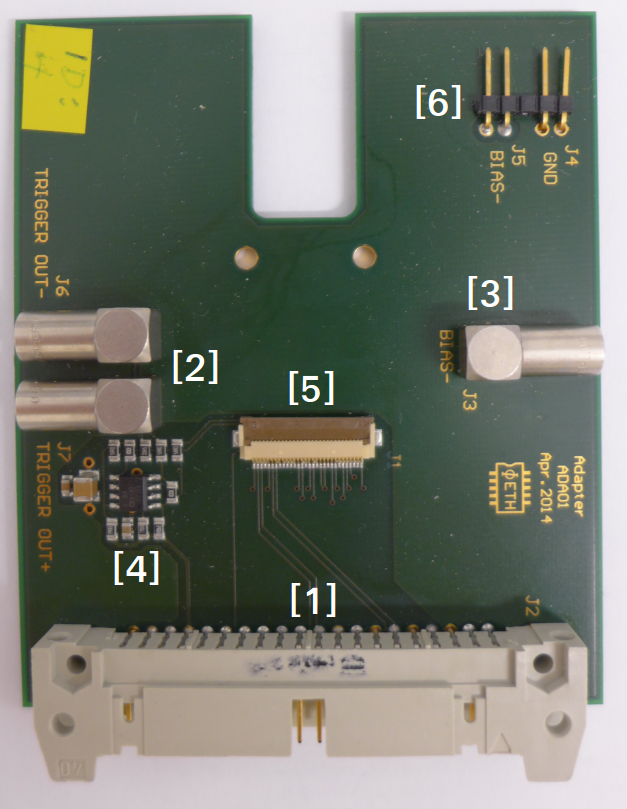
\includegraphics[width=0.47\textwidth]{setup/adaana1}\label{p4}}
	\hfill
	\subbottom[Version 2 with \ac{ROC} mounted underneath the black cover]{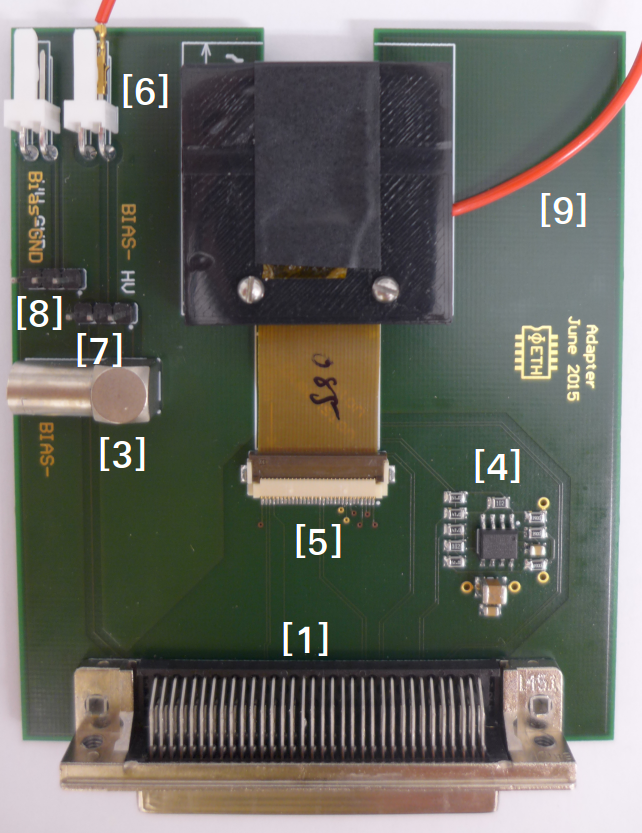
\includegraphics[width=0.47\textwidth]{setup/adaana2}\label{p5}}
	\caption{Analogue adapter planes of the two telescope versions.}
	\label{padaana}
\end{figure}\no
% ========================================================
